% Note for any github stalkers. I am currently in the process
% of learning LaTeX. I don't know what I'm doing yet. Sorry
% if my code absolutely sucks.

% Additional note for gihub stalkers. I'm sorry I haven't
% learned how to split this into multiple files yet. Sorry.


\documentclass{book}

\usepackage{fontspec} % used to import Calibri
\usepackage{anyfontsize} % used to adjust font size

% needed for inch and other length measurements
% to be recognized
\usepackage{calc}

% for colors and text effects as is hopefully obvious
\usepackage[dvipsnames]{xcolor}
\usepackage{soul}

% control over margins
\usepackage[margin=1in]{geometry}
\usepackage[strict]{changepage}

\usepackage{mathtools}
\usepackage{amsfonts}
\usepackage{amssymb} % originally imported to get the proof square
\usepackage[overcommands]{overarrows} % Get my preferred vector arrows...
\usepackage{xfrac}
\usepackage{relsize}

% Just am using this to get a dashed line in a table...
% Also you apparently want this to be inactive if you aren't
% using it because it slows compilation.
\usepackage{arydshln} \ADLinactivate 
\newenvironment{allowTableDashes}{\ADLactivate}{\ADLinactivate}

\usepackage{graphicx}
\graphicspath{{./140A_images/}}

\usepackage{tikz}
   \usetikzlibrary{arrows.meta}

\newfontfamily{\calibri}{Calibri}


\setlength{\parindent}{0pt}
\definecolor{RawerSienna}{HTML}{945D27}

\newcommand{\hOneOld}{%
   \color{Black}%
   \fontsize{14}{14}\selectfont%
}
\newcommand{\hOne}{%
   \color{Black}%
   \fontsize{14}{16}\selectfont%
}
\newcommand{\hTwoOld}{% deprecated
   \color{MidnightBlue}%
   \fontsize{13}{13}\selectfont%
}
\newcommand{\hTwo}{%
   \color{MidnightBlue}%
   \fontsize{13}{15}\selectfont%
}
\newcommand{\hThreeOld}{% deprecated
   \color{PineGreen}
   \fontsize{13}{13}\selectfont%
}
\newcommand{\hThree}{%
   \color{PineGreen}
   \fontsize{13}{15}\selectfont%
}
\newcommand{\hFour}{%
   \color{Cerulean}
   \fontsize{12}{14}\selectfont%
}
\newcommand{\myComment}{%
   \color{RawerSienna}%
   \fontsize{12}{14}\selectfont%
}
\newcommand{\teachCommentOld}{% deprecated
   \color{Orange}%
   \fontsize{12}{12}\selectfont%
}
\newcommand{\teachComment}{
   \color{Orange}%
   \fontsize{12}{14}\selectfont%
}
\newcommand{\exOne}{%
   \color{Purple}%
   \fontsize{14}{14}\selectfont%
}
\newcommand{\exP}{%
   \color{VioletRed}%
   \fontsize{12}{12}\selectfont%
}

\newenvironment{myIndent}{%
   \begin{adjustwidth}{2.5em}{0em}%
}{%
   \end{adjustwidth}%
}
\newenvironment{myDindent}{%
   \begin{adjustwidth}{5.0em}{0em}%
}{%
   \end{adjustwidth}%
}
\newenvironment{myTindent}{%
   \begin{adjustwidth}{7.5em}{0em}%
}{%
   \end{adjustwidth}%
}

\newcommand{\udefine}[1]{%
   \setulcolor{Red}%
   \setul{0.14em}{0.07em}%
   \ul{#1}%
}

\newcommand{\uuline}[2][.]{%
{\vphantom{a}\color{#1}%
\rlap{\rule[-0.18em]{\widthof{#2}}{0.06em}}%
\rlap{\rule[-0.32em]{\widthof{#2}}{0.06em}}}%
#2}

\newcommand{\fillInBlank}[2][.]{{%
   \color{#1}%
   \rule[-0.12em]{#2em}{0.06em}\rule[-0.12em]{#2em}{0.06em}%
   \rule[-0.12em]{#2em}{0.06em}
}}

\newcommand{\retTwo}{\hfill\bigbreak}

\newcounter{LectureNumber}
\newcommand*{\markLecture}[1]{%
   \stepcounter{LectureNumber}%
   {\huge \color{Black} \textbf{Lecture \theLectureNumber: #1} \newline}%
}

\newcommand{\pprime}{\prime\prime}

\newcommand{\rea}[1]{\mathrm{Re}(#1)}
\newcommand{\ima}[1]{\mathrm{Im}(#1)}


\newcounter{PropNumber}
\newcommand{\propCount}[1][1]{%
   \addtocounter{PropNumber}{#1}%
   \thePropNumber%
}
\newcounter{SubPropNumber}
\newcommand{\subPropCount}[1][1]{%
   \addtocounter{SubPropNumber}{1}%
   \theSubPropNumber%
}
\newcommand{\resetSubPropCount}{%
   \setcounter{SubPropNumber}{0}%
}


\newcommand{\mySepOne}[1]{%
   {\noindent\color{#1}{\rule{6.5in}{1mm}}}\\%
}
\newcommand{\mySepTwo}[1][.]{%
   {\noindent\color{#1}{\rule{6.5in}{0.5mm}}}\\%
}

\newenvironment{myClosureOne}[2][.]{%
   \color{#1}%
   \begin{tabular}{|p{#2in}|} \hline \\%
}{%
   \\ \\ \hline \end{tabular}%
}

% Overarrow stuff:
% ~~~~~~~~~~~~~~~~~~~~~~~~~~~~~~~~~~~~~~~~~~~~~~~~~~~~~~~~~~
\NewOverArrowCommand{myVector}{%
   start = {{\smallermathstyle\relbar}},
   middle = {{\smallermathstyle\relbareda}},
   end={{\rightharpoonup}}, space before arrow=0.15em,
   space after arrow=-0.045em,
}

\NewOverArrowCommand{myBar}{%
   start = {{\smallermathstyle\relbar}},
   middle = {{\smallermathstyle\relbar}},
   end={{\relbar}}, space before arrow=0.15em,
   space after arrow=-0.025em,
}

% ~~~~~~~~~~~~~~~~~~~~~~~~~~~~~~~~~~~~~~~~~~~~~~~~~~~~~~~~~~~~

\newcommand{\mVec}[1]{\myVector{#1}}
\newcommand{\mMat}[1]{\mathbf{#1}}

\title{Math 140A Lecture Notes (Professor: Brandon Seward)}
\author{Isabelle Mills}


\begin{document}
   \maketitle
   \calibri

   \markLecture{1/8/2024}

   \hOneOld
   An \udefine{order} on a set $S$, typically denoted as $<$, is
   a binary relation satisfying:
   \begin{enumerate}
      \item $\forall x, y \in S$, exactly one of the following is true:
      \begin{itemize}
         \item $x<y$ \item $x=y$ \item $y<x$
      \end{itemize}

      \item given $x, y, z \in S$, we have that $x<y<z\Rightarrow x<z$
   \end{enumerate}
   \hfill \bigbreak

   As a shorthand, we will specify that
   \begin{itemize}
      \item $x>y \Leftrightarrow y<x$
      \item $x\leq y \Leftrightarrow x<y \text{ or } x=y$
      \item $x\geq y \Leftrightarrow x>y \text{ or } x=y$
   \end{itemize}

   An \udefine{ordered set} is a set with a specified ordering. Let
   $S$ be an ordered set and $E$ be a nonempty subset of $S$. 

   \hTwoOld
   \begin{myIndent}
   \begin{itemize}
      \item If $b \in S$ has the property that $\forall x \in E, \hspace{0.25em}
      x \leq b$, then we call $b$ an\\ \udefine{upperbound} to $E$ and 
      say that $E$ is \udefine{bounded above} by $b$.
      \hfill \bigbreak
      
      \item if $b \in S$ has the property that $\forall x \in E, 
      \hspace{0.25em} x \geq b$, then we call $b$ an 
      \udefine{lower bound} to $E$ and say that $E$ is 
      \udefine{bounded below} by $b$.
      \hfill \bigbreak
   
      \item We call $\beta \in S$ the \udefine{least upperbound} to $E$ if
      $\beta$ is an upper bound to $E$ and $\beta$ is the least of all
      upperbounds to $E$. In this case, we also commonly call $\beta$ 
      the \udefine{supremum} of $E$ and denote it as $\sup{E}$.
      \hfill \bigbreak
   
      \item We call $\beta \in S$ the \udefine{greatest lower bound} to $E$ if
      $\beta$ is an lower bound to $E$ and $\beta$ is the greatest of all
      lower bounds to $E$. In this case, we also commonly call $\beta$ 
      the \udefine{infimum} of $E$ and denote it as $\inf{E}$.
      \hfill \bigbreak

      \item We call $e \in E$ the \udefine{maximum} of E if $\forall 
      x \in E, \hspace{0.25em} x \leq e$
      \hfill \bigbreak

      \item We call $e \in E$ the \udefine{minimum} of E if $\forall 
      x \in E, \hspace{0.25em} x \geq e$
      \hfill \bigbreak
   \end{itemize}
   \end{myIndent}

   \hOneOld
   \uuline{Fact}: For an ordered set $S$ and nonempty $E\subseteq S$,
   either:
   \begin{itemize}
      \item neither $\max{E}$ nor $\sup{E}$ exists
      \item $\sup{E}$ exists but $\max{E}$ does not exist
      \item $\max{E}$ exists and $\sup{E}=\max{E}$
   \end{itemize}

   \pagebreak
   \exOne
   Using $\mathbb{Q}$ as our ordered set...
   \begin{itemize}
      \item For $E = \{q \in \mathbb{Q} \mid 0<q<1\}$,
      $\max{E}$ does not exist but $\sup{E}$ exists and equals $1$.
      \exP
      \begin{myIndent}
         To understand why, note that the set of all upper bounds
         of $E$ is equal to\\ $\{q \in \mathbb{Q} \mid q \geq 1\}$ and 
         $1$ is obviously the smallest element of that set. Thus, $1$
         is the supremum of $E$. However, $1 \notin E$. Thus, if
         $\max{E}$ did exist, it would have to not equal $1$. But that
         would contradict $1$ being the least greatest bound.
      \end{myIndent}
      \hfill \bigbreak

      \exOne
      \item For $E = \{q \in \mathbb{Q} \mid 0<q \leq 1\}$,
      $\max{E}$ and $\sup{E}$ exist and they both are equal to $1$
      \exP
      \begin{myIndent}
         The reasoning for this is similar to that for the previous set.
      \end{myIndent}
      \hfill \bigbreak
      
      \exOne
      \item For $E = \{q \in \mathbb{Q} \mid q^2 < 2\}$, neither
      $\max{E}$ and $\sup{E}$ exist.
      \exP
      \begin{myIndent}
         To prove this, we can show there exists a function $f:
         \mathbb{Q}^+\rightarrow\mathbb{Q}^+$ such that
         $\forall q \in \mathbb{Q}^+$,\\ $q^2 < 2
         \Rightarrow q^2 < (f(q))^2 < 2$ and $2 < q^2
         \Rightarrow 2 < (f(q))^2 < q^2$. That way we can give
         a counter example to any possible claimed supremum or 
         maximum of $E$.
         \hfill \bigbreak


         Now instead of being like Rudin and simply providing the desired
         function, I want to present how one may come up with a function 
         that works for this proof themselves.
         \hfill \bigbreak

         Firstly, note that for the following reasons, we know our 
         desired function must be a rational function:
         \begin{itemize}
            \item[$\diamond$] $\forall q \in \mathbb{Q}, \hspace{0.25em} 
            f(q) \in \mathbb{Q}$. Based on this, we can't use any radicals,
            trig functions, logarithms, or exponentials in our desired
            function. \hfill \bigbreak

            \item[$\diamond$] $q^2 > 2 \Rightarrow f(q) < q$. In other
            words, $f$ needs to grow slower than a linear function. Thus,
            we can rule out the possibility of $f$ being a polynomial.
            \hfill \bigbreak

            \item[$\diamond$] If we wanted $f$ to be a linear function,
            it would have to have the form\\ $f(q) = \alpha(q - \sqrt{2})
            + \sqrt{2}$ where $\alpha$ is some constant. This is
            because when $q^2 = 2, \hspace{0.25em} f(q) = q$. However, there
            is no value one can set $\alpha$ to which both eliminates the
            presence of irrational numbers in that function while
            simultaneously making $f(q) \neq q$ when $q^2 \neq 2$. So
            no linear function can possibly work for this proof.
            \hfill \bigbreak
         \end{itemize}

         Having narrowed our search, let's now pick some convenient
         properties we would wish our proof function to have. Specifically,
         let's force $f$ to be constantly increasing, have a $y$-intercept
         of $1$, and approach a horizontal asymptote of $y = 2$. Doing this,
         we can now say that an acceptable function will have the following
         form where $\alpha$ is an unknown constant:
         \[f(q) = 1 + \frac{q}{q + \alpha}\]
         
         And finally, we can solve for $\alpha$ using the following system
         of equations:
         \[\begin{matrix}
            (1 + \frac{q}{q + \alpha})^2 = 2 \\
            \\
            1 + \frac{q}{q + \alpha} = q
         \end{matrix}\]

         Now here's where a graphing calculator like Desmos can be very
         useful. Instead of painstakely having to solve for $\alpha$,
         we can use a graphing calculator to approximate the value of
         $\alpha$ that satisfies our system of equations.
         \begin{center}
         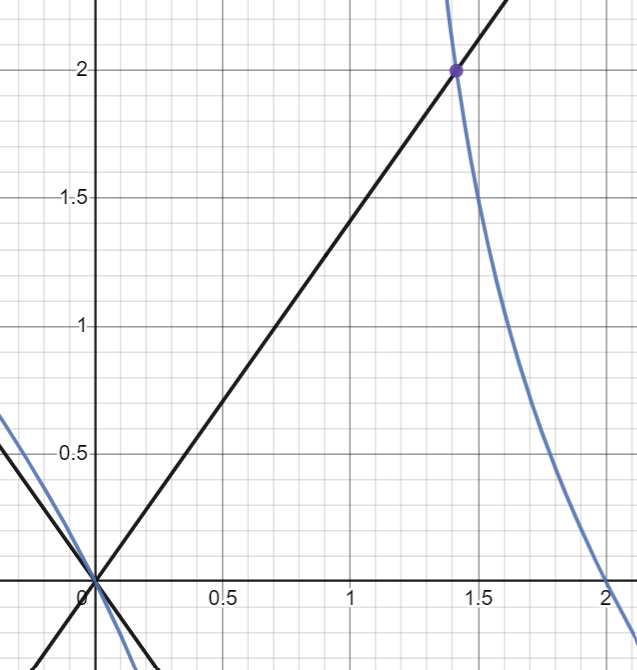
\includegraphics[scale=0.75]{Finding_Equation_Demonstration_1.png}
         \end{center}

         Based on the graph above, it looks like $f(q) = 1 +
         \frac{q}{q + 2}$ will work for our proof. And sure enough 
         it does. Furthermore, we can verify that the function we came
         up with is equivalent to that which Rudin presents.
      \end{myIndent}
   \end{itemize}

   \mySepOne{Purple}
   \hOneOld\hfill \break
   We say an ordered set $S$ has the \udefine{least upperbound
   property} if and only if when $E \subseteq S$ is nonempty and 
   bounded above, then the supremum of $E$ exists in $S$. Additionally, 
   we say an ordered set $S$ has the \udefine{greatest lower bound 
   property} if and only if when $E \subseteq S$ is nonempty and 
   bounded below, then the infimum of $E$ exists in $S$.
   
   \begin{myIndent}\begin{myIndent}\begin{myIndent}
   \begin{myIndent}\begin{myIndent}
      \teachCommentOld
      When we define the set of real numbers, this will be one of the
      fundamental properties of that set. \hfill \bigbreak
   \end{myIndent}\end{myIndent}\end{myIndent}
   \end{myIndent}\end{myIndent}

   \markLecture{1/10/2024}
   \begin{myIndent}
      \hTwoOld
      Proposition \propCount: $S$ has the least upperbound property if
      and only if $S$ has the greatest lower bound property.
      
      \hThreeOld
      \begin{myIndent}
         Proof: Let's say we have an ordered set $S$
         \hfill \bigbreak

         Assume $S$ has the least upperbound property. Then, let
         $B \subseteq S$ be a nonempty subset which is bounded below.
         Additionally, let $A \subseteq S$ be the set of all lower bounds
         of $B$. \newpage
         
         \begin{myIndent}
            We know that $A \neq \emptyset$ because we assumed that $B$ is
            bounded below. Thus, at least one lower bound to $B$ exists and
            belongs to $A$. \\Additionally, because we assumed $B$ is nonempty,
            we can say that each $b \in B$ is an upper bound to $A$. Thus, $A$
            is bounded above. Because of these two facts, we can apply the
            greatest lower bound property to say that the supremum of $A$ 
            exists. \hfill \bigbreak
   
            Let's define $\alpha \coloneq \sup{A}$. With that, our goal is 
            now to show that\\ $\alpha = \inf{B}$. To do this, we need to 
            show firstly that $\alpha$ is a lower bound to $B$ and 
            secondly that it is greater than all other lower bounds of $B$.
            \retTwo
            \begin{enumerate}
               \item For each $b \in B$, we have that $b$ is an 
                  upperbound to $A$. And since $\alpha = \sup{A}$ is the
                  least upperbound to $A$, we must have that $\alpha \leq
                  b$. Thus $\alpha$ is a lower bound to $B$. \retTwo
               
               \item If $x \in S$ is a lower bound to $B$, then $x \in A$.
                  And since\\ $\alpha = \sup{A}$, $x \leq \alpha$. This shows
                  that $\alpha$ is greater than or equal to all other lower
                  bounds. \retTwo
            \end{enumerate}
            
            Hence, $\alpha$ is the infimum of $B$. And since we did this
            for a general \\$B \subseteq S$, we can thus say that $S$ has
            the greatest lower bound property. \retTwo
         \end{myIndent}

         Now we skipped doing the reverse direction proof because it
         is almost completely identical to the foward direction proof.
         However, just know that the above proposition is an
         \uuline{if and only if} statement. $\blacksquare$
      \end{myIndent}
   \end{myIndent}

   \mySepOne{PineGreen}
   \hOneOld\hfill \break
   A \udefine{field} is a set $F$ equipped with $2$ binary operations,
   denoted $+$ and $\cdot$, and containing two elements $0 \neq 1 \in F$
   satisfying the following conditions for all $x, y, z \in F$:

   \hTwoOld
   \begin{myIndent}
      
      \begin{tabular}{ l c }%
         {\large \textbullet} \hspace{1ex} Associativity: &
            $\begin{matrix} (x + y) + z = x + (y + z) \\ (x \cdot y) 
               \cdot z = x \cdot (y \cdot z) \end{matrix}$ \\ \\
         
         {\large \textbullet} \hspace{1ex} Commutativity: &
            $\begin{matrix} x+y=y+x\\x\cdot y = y \cdot x\end{matrix}$
               \\ \\
         
         {\large \textbullet} \hspace{1ex} Identity: &
            $\begin{matrix}0+x=x\\1\cdot x=x\end{matrix}$ \\ \\
         
         {\large \textbullet} \hspace{1ex} Inverses: &
            $\begin{matrix} \forall x\in F, \hspace{0.5em}
               \exists {-x} \in F \hspace{0.50em} s.t.
               \hspace{0.50em} x + {-x} = 0 \\ \forall x\neq 0\in F, 
               \hspace{0.5em} \exists {\displaystyle 
               \frac{1}{x}} \in F \hspace{0.50em} s.t. \hspace{0.50em} 
               x \cdot {\displaystyle \frac{1}{x}}=1\end{matrix}$ \\ \\
         
         {\large \textbullet} \hspace{1ex} Distributivity: &
            $x \cdot (y + z) = (x \cdot y) + (x \cdot z)$
      \end{tabular}
   \end{myIndent}

   \newpage
   \hOneOld
   We shall assign the following notation: 
   
   {
      \hTwoOld %  Ok so I now know that lines on the table
            % at least by default have the same color as the
            % text color.
      \centering
      \renewcommand{\arraystretch}{2.2}
      \begin{allowTableDashes}
         \begin{tabular}{ c;{10pt/3pt}c }
         
            We write \fillInBlank{1} \hspace{0.75em} & 
               \hspace{0.75em} to mean \fillInBlank{1} \\ \hline
            
            $x-y$ & $x + {-y}$ \\ \hdashline[10pt/3pt]

            ${\displaystyle \frac{x}{y}}$ & $x \cdot 
                  {\displaystyle \frac{1}{y}}$\\[8pt] \hdashline[10pt/3pt]
            
            $2$ & $1 + 1$\\ \hdashline[10pt/3pt]

            $2x$ & $x + x$\\ \hdashline[10pt/3pt]

            $x^2$ & $x \cdot x$\\ \hdashline[10pt/3pt]

            $xy$ & $x\cdot y$
         \end{tabular}
      \end{allowTableDashes}
      \par
   }
   \retTwo
   
   \hOneOld
   Now what follows is a number of propositions concerning the 
   arithmetic properties of a field...
   
   \begin{myIndent}
      \hTwoOld
      \resetSubPropCount
      For a field $F$ and elements $x,y,z\in F$, we have the
      following propositions:
      
      Proposition \propCount.\subPropCount: $x+y=x+z \Rightarrow y=z$
      {\hThreeOld
      \begin{myIndent}
         Proof: Assume $x+y=x+z$. Then...
            \begin{myIndent}
               \renewcommand{\arraystretch}{1.4}
               \begin{tabular}{ l c }
                  $y=0+y$ & (addition identity property)\\
                  $\hphantom{y}=({-x}+x)+y$ & (addition inverse property)\\
                  $\hphantom{y}={-x}+(x+y)$ & (addition associative property)\\
                  $\hphantom{y}={-x}+(x+z)$ & (by our assumption)\\
                  $\hphantom{y}=({-x}+x)+z$ & (addition associative property)\\
                  $\hphantom{y}=0+z$ & (addition inverse property)\\
                  $\hphantom{y}=z$ & (addition identity property)
               \end{tabular}
            \end{myIndent}
      \end{myIndent} \retTwo}

      Proposition \propCount[0].\subPropCount: $x+y=x \Rightarrow y=0$
      {\hThreeOld
      \begin{myIndent}
         Proof: Plug in $z=0$ into proposition 2.1. in order to get
         that $y=z=0$.
      \end{myIndent} \retTwo}

      Proposition \propCount[0].\subPropCount: $x+y=0 \Rightarrow y={-x}$
      {\hThreeOld
      \begin{myIndent}
         Proof: Plug in $z={-x}$ into proposition 2.1. in order to get
         that\\ $y=z={-x}$.
      \end{myIndent} \retTwo}

      Proposition \propCount[0].\subPropCount: ${-(-x)}=x$
      {\hThreeOld
      \begin{myIndent}
         Proof: Observe that $x+{-x}={-x}+x=0$ by the inverse and\\ 
         commutative properties of addition. Then, by proposition
         2.3, we know that ${-x}+x=0 \Rightarrow x={-(-x)}$.
      \end{myIndent}}
      \newpage
      Proposition \propCount[0].\subPropCount: $x\cdot y=x\cdot z 
                                    \text{ and } x\neq0\Rightarrow y=z$
      {\hThreeOld
      \begin{myIndent}
         Proof: Assume $x\cdot y=x\cdot z$ and $x\neq0$. Then...
            \begin{myIndent}
               \renewcommand{\arraystretch}{1.4}
               \begin{tabular}{ l c }
                  $y=1\cdot y$ & (multiplication identity property)\\
                  $\hphantom{y}=(\frac{1}{x}\cdot x)\cdot y$ & 
                                 (multiplication inverse property)\\
                  $\hphantom{y}=\frac{1}{x}\cdot(x\cdot y)$ & 
                                 (multiplication associative property)\\
                  $\hphantom{y}=\frac{1}{x}\cdot(x\cdot z)$ & 
                                 (by our assumption)\\
                  $\hphantom{y}=(\frac{1}{x}\cdot x)\cdot z$ & 
                                 (multiplication associative property)\\
                  $\hphantom{y}=1\cdot z$ & 
                                 (multiplication inverse property)\\
                  $\hphantom{y}=z$ & 
                                 (multiplication identity property)
               \end{tabular}
               \retTwo
            
         \begin{myIndent}\begin{myIndent}\begin{myIndent}
            \teachCommentOld
            Note that to use the multiplication inverse\\ property,
            we have to assume $x \neq 0$ !!
         \end{myIndent}\end{myIndent}\end{myIndent}

         \end{myIndent}
      \end{myIndent} \retTwo}

      Proposition \propCount[0].\subPropCount: $x\cdot y=x \Rightarrow y=1$
      {\hThreeOld
      \begin{myIndent}
         Proof: Plug in $z=1$ into proposition 2.5. in order to get
         that $y=z=1$.
      \end{myIndent} \retTwo}

      Proposition \propCount[0].\subPropCount: $x\cdot y=1 \Rightarrow 
               y={\displaystyle\frac{1}{x}}$
      {\hThreeOld
      \begin{myIndent}
         Proof: Plug in $z={\frac{1}{x}}$ into proposition 2.5. in order to get
         that\\ $y=z={\frac{1}{x}}$.
      \end{myIndent} \retTwo}

      Proposition \propCount[0].\subPropCount:
         ${\dfrac{\hspace{0.15em}1\hspace{0.15em}}{
            \frac{1}{x}}} = x$
      {\hThreeOld
      \begin{myIndent}
         Proof: Observe that $x\cdot{\frac{1}{x}}=
         {\frac{1}{x}}\cdot x=1$ 
         by the inverse and commutative \\[3pt] properties of multiplication. 
         Then, by proposition 2.7, we know that \\[3pt]
         ${\frac{1}{x}}\cdot x=1 \Rightarrow x={
         \dfrac{\hspace{0.15em}1\hspace{0.15em}}{\frac{1}{x}}}$.
      \end{myIndent} \retTwo}

      Proposition \propCount[0].\subPropCount: $0\cdot x = 0$
      {\hThreeOld
      \begin{myIndent}
         Proof: $(0\cdot x) + (0\cdot x) = (0+0)\cdot x = 0\cdot x$.
         Thus we have an expression of the form $a+b=a$ which we can use
         proposition 2.2 on. Hence, we can conclude $0\cdot x=0$.
      \end{myIndent} \retTwo}

      Proposition \propCount[0].\subPropCount: 
         $x\neq0 \text{ and } y\neq0 \Rightarrow x\cdot y \neq 0$
      {\hThreeOld
      \begin{myIndent}
         Proof: since $x, y\neq0$, we can say that $x\cdot y \cdot
         {\frac{1}{x}} \cdot {\frac{1}{y}}
         = 1 \neq 0$. Now by proposition 2.9, $x\cdot y=0 \Rightarrow
         (x\cdot y)\cdot\left({\frac{1}{x}} \cdot 
         {\frac{1}{y}}\right)=0$. However, we know that is not the
         case. So $x\cdot y$ can't equal zero.
      \end{myIndent} \retTwo}
   \end{myIndent}
   \newpage
   
   \markLecture{1/12/2024}
   
   {\begin{myIndent} \hTwo
   Proposition \propCount[0].\subPropCount: $({-x})y={-(xy)}=x({-y})$
      {\hThree
      \begin{myIndent}
         Proof: $xy+({-x})y=(x+{-x})y=0y=0$. Thus by proposition 2.3,\\
         $({-x})y={-(xy)}$. We can make a similar argument to also say
         that\\ $x({-y})={-(xy)}$.
      \end{myIndent} \retTwo}

      Proposition \propCount[0].\subPropCount: $({-x})({-y})=xy$
      {\hThree
      \begin{myIndent}
         Proof: Using proposition 2.11, we can say that \\
         $({-x})({-y}) = {-(x({-y}))} = {-({-(xy)})}$. Then
         by proposition 2.4, we can \\conclude ${-({-(xy)})} = xy$.
      \end{myIndent} \retTwo}
   \end{myIndent}}
   
   \mySepOne{Black}


   An \udefine{ordered field} is a field $F$ equipped with an ordering
   $<$ satisfying $\forall x,y,z \in F$:
   
   \begin{myIndent}\begin{myIndent}
      \begin{enumerate}
         \item[OF1.] $y<z \Rightarrow y+x<z+x$
         \item[OF2.] $(x>0 \text{ and } y>0) \Rightarrow xy>0$ 
      \end{enumerate}
   \end{myIndent}\end{myIndent} \retTwo

   For $x$ in an ordered field, we call $x$ \udefine{positive} if and 
   only if $x>0$. Similarly, we call $x$ \udefine{negative} if and
   only if $x<0$.

   {\begin{myIndent} \hTwo
   Proposition \propCount: For an ordered field $F$ and 
      $x, y, z \in F$, we have:

      \begin{enumerate}
         \item $x<y \Leftrightarrow {-y}<{-x}$
         {\begin{myIndent} \hThree
            Proof: By property OF1 of an ordered field, we can
            say that\\ $x<y\Rightarrow x+({-x}+{-y})<y+({-x}+{-y})
            \Rightarrow -y < -x$. \retTwo
         \end{myIndent}}

         \item $(x>0 \text{ and } y<z) \Rightarrow xy<xz$
         {\begin{myIndent} \hThree
            Proof: By property OF1 of an ordered field, $y<z
            \Rightarrow y-y<z-y$. Or in other words, $0<z-y$.  
            Therefore, since $x$ is also positive by assumption,
            property OF2 of an ordered field tells us that
            $x(z-y)>0$. Finally, adding $xy$ to both sides by property
            OF1 and then distributing gives us: \\$xz-xy+xy=xz<xy$.
            \retTwo
         \end{myIndent}}

         \item $(x<0 \text{ and } y<z) \Rightarrow xy>xz$
         {\begin{myIndent} \hThree
            Proof: Since $x<0$, we have $-x>0$ by proposition 3.1.
            Then by applying proposition 3.2, we know that
            $(-x>0 \text{ and } y<z) \Rightarrow -xy<-xz$.
            Finally, by reapplying proposition 3.1, this becomes
            $xy>xz$.\retTwo
         \end{myIndent}}

         \item $x \neq 0 \Rightarrow x^2 > 0$
         {\begin{myIndent} \hThree
            Proof: If $x>0$, then $x^2=xx>0x=0$ by property OF2
            of an \\ordered field. Meanwhile, if $x<0$, then $-x>0$
            by proposition 3.1. So $(-x)(-x)>0$ by property OF2.
            But $(-x)(-x)=x^2$ by proposition 2.12. So $x^2>0$.
            \retTwo
         \end{myIndent}}
         \newpage

         \item $0<x<y \Rightarrow 0<\frac{1}{y}<\frac{1}{x}$
         {\begin{myIndent} \hThree
            Proof: Since $y>0$ and $y\cdot\frac{1}{y}=1>0=0\cdot\frac{1}{y}$,
            we must have $\frac{1}{y}>0$ by propositions 3.2 and 3.3.
            Note that $\frac{1}{y}\neq0$ because if it did,
            $y\cdot\frac{1}{y}=0$. \\ Similarly, we can show $\frac{1}{x}
            >0$. Now multiply both sides of $x<y$ by the positive element
            $\frac{1}{x}\cdot\frac{1}{y}$ and apply proposition 3.2
            to get that $\frac{1}{y}<\frac{1}{x}$.
            \retTwo
         \end{myIndent}}
      \end{enumerate}
   \end{myIndent}}

   \mySepTwo[Black]

   \hOne
   \uuline{Theorem}: There is (up to isomorphism) precisely one ordered field that contains $\mathbb{Q}$ and has the least upper bound property.
   We denote this field $\mathbb{R}$ and we call its elements 
   \udefine{real numbers}.
   
   \begin{myIndent}\begin{myIndent}\begin{myIndent}\begin{myIndent}
   \begin{myIndent}\begin{myIndent}
      {\teachComment
         In other words, this theorem is stating that $\mathbb{R}$ exists and is unique. Unfortunately, the proof for this is very long and so won't be covered in lecture. However, the professor has left some resources to cover it. So, I will have the proof of this theorem later in these notes. \newline
            See page: {\color{BrickRed} <research how to cite a page>}
      }
   \end{myIndent}\end{myIndent}
   \end{myIndent}\end{myIndent}\end{myIndent}\end{myIndent}

   \mySepTwo[Black]

   
   {\begin{myIndent} \hTwo \resetSubPropCount
      Proposition \propCount.\subPropCount: If $x\in\mathbb{R}$, $y\in\mathbb{R}$, and $x>0$, then there is a positive integer $n$ such that $nx>y$. This is called the \udefine{archimedean property}.

      {\begin{myIndent} \hThree
         Proof: We proceed by looking for a contradiction. Let $A=\{nx \mid n\in\mathbb{Z}^+\}$ and assume $\nexists n\in\mathbb{Z}^+$ such that $nx>y$. In that case we know $y$ is an \\upper bound of $A$. Additionally, since $A$ is bounded above, we know by the least upper bound property of the real numbers that $\sup{A}$ exists. So, let $\alpha=\sup{A}$. \retTwo

         Now because $\mathbb{R}$ is an ordered field, we know that: \\
         $x>0 \Rightarrow -x<0 \Rightarrow \alpha-x<\alpha$. Therefore, because $\alpha$ is the least upper bound, we know that $\alpha - x$ is not an upper bound for $A$. Or in other words, there exists $n\in\mathbb{Z}^+$ such that $nx>\alpha-x$. But this contradicts that $\alpha$ is the least upper bound of $A$ because $nx>\alpha-x \Rightarrow (n+1)x>\alpha$ and $(n+1)x\in A$. So we conclude that the supremum of $A$ can't exist, which by the contrapositive of the least upper bound property, means that $A$ is not bounded above.
         \retTwo
      \end{myIndent}}

      Proposition \propCount[0].\subPropCount: If $x, y\in\mathbb{R}$ and $x<y$, then there exists a $p\in\mathbb{Q}$ such that\\ $x<p<y$. In other words, we say that $Q$ is \udefine{dense} in $R$.

      {\begin{myIndent} \hThree
         Proof: Since $x<y$, we have that $0<y-x$. Then because $y-x$ is positive, we can use the archimedean property to say that there exists an integer $n$ such that $n(y-x)>1$. Note for later that this means $ny>1+nx$.

         \newpage

         Now note that since $1>0$ and $nx$ is a real number, we can use the archimedean property twice to get positive integers $m_1$ and $m_2$ such that $m_1\cdot1>-nx$ and $m_2\cdot1>+nx$. Thus, we get the expression $-m_1 < nx < m_2$. So now \\consider the set $B = \{m \in \mathbb{Z} \mid -m_1 \geq nx \geq m_2 \text{ and } m>nx\}$. We know that $B$ has finitely many elements and that $B$ contains at least one \\element: $m_2$. So $B$ must have a minimum element. We'll refer to that \\minimum element as $m$. Notably, as $m$ is the minimum element of $B$, we know that $m-1 \notin B$, meaning that $m-1\leq nx < m$ \retTwo

         We now combine inequalities as follows: $m-1 \leq nx \Rightarrow m \leq nx+1$. So we have that $nx < m \leq nx+1$. But now remember from the previous page that $ny>1+nx$. So we can say that $nx < m \leq nx+1 < ny$. Finally, because $n>0$, we can multiply the inequality by $\frac{1}{n}$ to get that $x<\frac{m}{n}<y$. $\blacksquare$

      \end{myIndent}}
   \end{myIndent}}
   \mySepTwo \newline
   \markLecture{1/17/2024} \newline
   \uuline{Theorem}: If $x\in\mathbb{R}$, $x>0$, $n\in\mathbb{Z}$, and $n>0$, then there is a unique $y\in \mathbb{R}$ with $y>0$ and $y^n=x$. This number $y$ is denoted $\sqrt[n]{x}$ or $x^\frac{1}{n}$. \retTwo

   {\begin{myIndent} \hTwo
      To prove this, first note the following lemma about positive integers $n$ and $a, b\in\mathbb{R}$:
      
      {\centering $b^n-a^n=(b-a)(b^{n-1}+ab^{n-2}+\ldots+a^{n-2}b+a^{n-1})$ \par}

      To prove this, one can either use induction or just calculate it out by hand to verify that the equality holds. \retTwo

      Additionally, also consider that if $n$ is a positive integer and $0\leq a \leq b$ where \\ $a,b\in\mathbb{R}$, then we have that $a^n\leq b^n$. Combining this fact with the lemma above, we can say that $0\leq a \leq b$ implies that $b^n-a^n \leq (b-a)nb^{n-1}$. Or in other words: $a^n \leq b^n \leq a^n + (b-a)nb^{n-1}$.
      {\teachComment  \begin{myTindent}\begin{myDindent}
         This comes from replasing every $a$ in the expression \\$(b^{n-1}+ab^{n-2}+\ldots+a^{n-2}b+a^{n-1})$ with $b$ in order to get that $b^n-a^n \leq (b-a)(b^{n-1} + b^{n-1} + \ldots + b^{n-1})$
      \end{myDindent}\end{myTindent}} \retTwo

      Now set $E=\{t\in\mathbb{R} \mid t>0, t^n\leq x\}$.
      {\begin{myIndent} \hThree
         We can show that $E$ is nonempty...
         \begin{itemize}
            \item If $x \geq 1$, then $t=1 \in E$ since $1^n=1\leq x$.
            \item If $x < 1$, then $x\in E$ since $x<1 \Rightarrow x^{n-1}<1^{n-1}=1$. But then $x^n<x$.
         \end{itemize}
         Thus, we know $E \neq \emptyset$. \retTwo

         We can also show that $E$ is bounded above. Consider $t=1+x$. In that case, $t>1$, which implies that $t^{n-1} > 1^{n-1} = 1$. Therefore, $t^n > t$, meaning that $t^n > x$. So $t=x+1$ is an upper bound for $E$.
         \newpage
         Thus by the least upper bound property of the real numbers, we know \\$y = \sup{E}$ exists. \retTwo
      \end{myIndent}}

      \uuline{Claim 1}: $y^n \geq x$.
      
      {\begin{myIndent} \hThree
         To prove this, we shall procede towards a contradiction. Assume $y^n<x$\retTwo
         
         Then pick some $h$ such that $0<h<\gamma$ and $\gamma$ is some mystery constant for us to find. Then, we can say that $y<y+h$, meaning by the lemma on the previous page that $y^n \leq (y+h)^n \leq y^n + (y+h-y)n(y+h)^n-1$. Or in other words, $(y+h)^n \leq y^n + hn(y+h)^n-1$. \retTwo

         Now we shall make our first assumption about $\gamma$: let $\gamma \leq 1$. That way, we know that $(y+h)^n \leq y^n + hn(y+h)^n-1 < y^n + hn(y+1)^n$. And since, we are assuming that $y^n<x$, we know there must exist some value of $h$ such that $y^n + hn(y+1)^{n-1} < x$. Putting this limitation on $h$, we get that $h < \frac{x - y^n}{n(y+1)^{n-1}}$ (Remember that $x-y^n$, $y$, and $n$ are all positive). So finally, we say that $\gamma = \min{\left( 1, \frac{x - y^n}{n(y+1)^{n-1}} \right)}$. This is so that for $0<h<\gamma$, we have that $(y+h)^n < x$. \retTwo

         Thus, we have a contradiction as we assumed that $y$ is the supremum of $E$ and yet we just proved that $y+h \in E$. So, $y^n$ cannot be less than $x$, meaning that that $y^n \geq x$. \retTwo
      \end{myIndent}}

      \uuline{Claim 2}: $y^n \leq x$.
      
      {\begin{myIndent} \hThree
         To prove this, we shall again proceed towards a contradiction. Assume \\$y^n>x$. \retTwo

         Then for some $h$ such that $0<h<\gamma$ where $\gamma$ is a new mystery constant, consider $y-h$. \retTwo

         
         {\begin{center} \hFour
            \begin{myClosureOne}{5}
               I now realize that I need to prove this lemma: for a positive integer $n$ and real numbers $a$ and $b$ such that $a \geq b$, we have that \\$(a-b)^n \geq a^n-bna^{n-1}$. We can prove this through induction. \\ \\
               Firstly for $n=1$: we have that $(a-b)^1 = a^1 - b(1)a^0$. \\ \\
               Now assume that for $k\geq 1$, $(a-b)^k \geq a^k - bka^{k-1}$.\\ Then $(a-b)^{k+1} = (a-b)(a-b)^k$. And since $(a-b)>1$, we know that $(a-b)^{k+1} = (a-b)(a-b)^k \geq (a-b)(a^k - bka^{k-1})$. \\ \\

               Now let's expand out our lesser term to get that: \\ $(a-b)^{k+1} \geq a^{k+1}-bka^k - ba^k + b^2ka^{k-1}$. Thus, we know that \\$(a-b)^{k+1} \geq a^{k+1}-b(k+1)a^k + b^2ka^{k-1} > a^{k+1}-b(k+1)a^k$. Hence, we have shown that $(a-b)^{k+1} \geq a^{k+1}-b(k+1)a^k$.
            \end{myClosureOne}
         \end{center}}
         \newpage

         Based on the lemma covered right before this, we have that \\$(y-h)^n \geq y^n-hny^{n-1}$. But now let's require that $y^n-hny^{n-1}>x$. Thus, we can say that $h<\frac{y^n-x}{ny^{n-1}}$. \retTwo

         So setting $\gamma = \frac{y^n-x}{ny^{n-1}}$, we have that for $0 < h < \gamma$, \hspace{0.25em} $(y-h)^n > x$. But this now leads to a contradiction as $y-h$ must be an upper bound to $E$.
         {\begin{myIndent} \hFour
            (If some number $z$ is greater than $y{-h}$, than $z^n > (y{-h})^n > x$. So $z \notin E$.) \newline
         \end{myIndent}}
         However, $y-h$ can't be an upper bound to $E$ as we specified that $y$ is the least upper bound of $E$. So we conclude that $y^n$ cannot be greater than $x$, thus meaning $y^n \leq x$.
      \end{myIndent}}

      So since $y^n \leq x$ and $y^n \geq x$, we conclude that $y^n = x$.
      \retTwo

      Finally, we now shall mention that $y$ is obviously the unique number such that \\$y^n=x$. After all, for $0<a<y<b$, we have that $a^n < y^n < b^n$. So, there can only be one number $y$ such that $y^n=x$.
   \end{myIndent}}

   \mySepTwo \newline
   \markLecture{1/19/2024}

   \uuline{Decimal representations of real numbers}:
   \begin{itemize}
      \item Each $x \in \mathbb{R}$ such that $x>0$ can be written $x=n_0.n_1n_2n_3\ldots$ where $n_0 \in \mathbb{Z}$ and $\forall i \geq 1$, $n_i \in \{0,1,2,3,4,5,6,7,8,9\}$.
      {\begin{myIndent} \hTwo
         Specifically, let $n_0$ be the largest integer with $n\leq x$. Then inductively, pick $n_k$ to be the max element in $\{0,1,2,3,4,5,6,7,8,9\}$ such that: \[
            n_0 + \frac{n_1}{10} + \cdots + \frac{n_{k-1}}{10^{k-1}} + \frac{n_k}{10^k} \leq x\]
      \end{myIndent}}
      
      \item Conversely, suppose $n_0 \in \mathbb{Z}$ and $\forall i \geq1, n_i \in \{0,1,2,3,4,5,6,7,8,9\}$. Then, defining $E=\{n_0, n_0 + \frac{n_1}{10}, \ldots, n_0 + \frac{n_1}{10} + \cdots + \frac{n_k}{10^k}, \ldots\}$, we have that\\ $n_0.n_1n_2n_3\ldots = x\in\mathbb{R}$ where $x = \sup{E}$.
   \end{itemize} \retTwo

   We will rarely ever use decimal representations though.

   \newpage

   The \uuline{extended real number system} is the set $\mathbb{R} \cup \{{-\infty}, {+\infty}\}$ where for all $x\in\mathbb{R}$:
   {\hTwo \begin{tabular}{ p{1.7in} p{2.2in} p{2.2in} }
      \begin{itemize}
         \item $-\infty < x < +\infty$
         \item $x + \infty = +\infty$
         \item $x - \infty = {-\infty}$
         \item $\frac{x}{+\infty} = 0 = \frac{x}{-\infty}$
      \end{itemize}
      &
      \begin{itemize}
         \item $x>0 \Rightarrow x(+\infty)=+\infty$
         \item $x>0 \Rightarrow x(-\infty)=-\infty$
         \item $+\infty +\infty = +\infty$
         \item $+\infty(+\infty) = +\infty$ 
      \end{itemize}
      &
      \begin{itemize}
         \item $x<0 \Rightarrow x(+\infty)=-\infty$
         \item $x<0 \Rightarrow x(-\infty)=+\infty$
         \item $-\infty - \infty = -\infty$
         \item $+\infty(-\infty) = -\infty$ 
      \end{itemize}
   \end{tabular}}
   {\begin{myTindent} \hFour
      All other operation involving $+\infty$ and $-\infty$ are left undefined. \retTwo
   \end{myTindent}}

   \diamond \hspace{0.5em} Sometimes, we denote the extended real number system $\overbar{\mathbb{R}}$.

   \diamond \hspace{0.5em} The extended real number system is not a field.

   \diamond \hspace{0.5em} To distinguish $x\in\mathbb{R}$ from $\infty$ or $-\infty$, we call $x\in\mathbb{R}$ finite.

   \mySepTwo

   The set of \udefine{complex numbers}, denoted $\mathbb{C}$, is the set of all things of the form $a+bi$ where $a, b \in \mathbb{R}$ and $i$ is a symbol satisfying $i^2=-1$.
   
   {\teachComment \begin{myTindent}\begin{myIndent}
      To be more rigorous about this definition, what we would do is define the set of complex numbers to be the set of pairs of real numbers equipped with the following operations:
      \begin{myIndent}
         For $z, u \in \mathbb{C}$ such that $z=(a, b)$ and $u=(c, d)$:
         \begin{itemize}
            \item $z+u = (a+c, b+d)$
            \item $z\cdot u = (ac - bd, ad+bc)$ \newline
         \end{itemize}
      \end{myIndent}
      Having done that, we would then:
      \begin{enumerate}
         \item Define $0 = (0, 0)$ and $1 = (1, 0)$
         \item Prove that $\mathbb{C}$ satisfies our field axioms
         \item Say that $i = (0, 1)$ and then show that $i^2 = (-1, 0)$
         \item And finally show that for $a, b \in \mathbb{R}$, \hspace{0.25em} $a(1) + b(i) = (a, b)$ 
         
         \begin{myTindent}\begin{myTindent}
            (Thus it makes sense to denote $z \in \mathbb{C}$ as $z = a + bi$)
         \end{myTindent}\end{myTindent} \retTwo
      \end{enumerate}

      However, we're behind and so not going to spend time doing that in class. \retTwo
   \end{myIndent}\end{myTindent}}
   
   For $z= a+bi$, we denote $\rea{z} = a$ the \udefine{real} part of $z$. On the other hand, we denote $\ima{z} = b$ the \udefine{imaginary} part of $z$. \retTwo

   The \udefine{complex conjugate} of $z=a+bi$ is $\overbar{z}=a-bi$.
   \newpage
   
   \begin{tabular}{ p{3.2in} p{2.8in} }
      {\hTwo \begin{myIndent}
         Proposition \propCount: If $z, w \in \mathbb{C}$, then:
         \begin{enumerate}
            \item $\overbar{z+w}=\overbar{z}+\overbar{w}$
            \item $\overbar{zw} = \overbar{z}\cdot \overbar{w}$
            \item $z + \overbar{z} = 2\rea{z}$
            \item $z - \overbar{z} = 2\ima{z}i$
            \item $z\overbar{z} \in \mathbb{R}$ and $z\overbar{z} > 0$ when $z\neq 0$. 
         \end{enumerate}
      \end{myIndent}}
      &
      \hThree
      \begin{myClosureOne}{2.8}
         {Proof: \newline
            \hFour
            Points 1-4 can be verified by direct\newline computation.\newline  As for point 5, note that if $z = a+bi$, then\newline $z\overbar{z} = (a+bi)(a-bi) = a^2+b^2$.\newline Now as $a, b\in\mathbb{R}$, we know that \newline $a^2+b^2\in\mathbb{R}$. But $a^2+b^2 > 0$ if $b\neq a\neq0$. Meanwhile, $a^2+b^2=0$ if $a=b=0$. So $z\overbar{z} > 0$ if $z\neq0$
         }
      \end{myClosureOne}
   \end{tabular} \retTwo
   
   The \udefine{absolute value} of $z=a+bi$ is $\lvert z\rvert = \sqrt{z\myBar{z}}$

   \begin{myIndent} \hTwo
      Propostion \propCount: For $z, w \in \mathbb{C}$, we have that:

      \begin{enumerate}
         \item $\lvert 0 \rvert = 0$ and $\lvert z \rvert > 0$ when $z\neq0$.
         \item $\lvert z \rvert = \lvert \overbar{z} \rvert$
         \item $\lvert zw \rvert = \lvert z \rvert\lvert w \rvert$
         \item $\lvert \rea{z} \rvert \leq \lvert z \rvert$
         \item $\lvert \ima{z} \rvert \leq \lvert z \rvert$
         \item $\lvert z + w \rvert \leq \lvert z \rvert + \lvert w \rvert$
         {\begin{myDindent} \teachComment
            This last bullet is the \uuline{triangle inequality}.
         \end{myDindent}}
      \end{enumerate}

      {\begin{myIndent} \hThree
         Proof:\\
         Claims 1, 2, and 3 can be verified through direct computation. \retTwo

         To prove claim 4, note that $a^2 \leq a^2+b^2$. So, $\lvert a \rvert = \sqrt{a^2} \leq \sqrt{a^2+b^2} = \lvert z \rvert$. We can repeat this but with $b^2$ to prove claim 5. \retTwo

         Lastly, to prove claim 6, note that $\lvert z+w\rvert^2=(z+w)(\overbar{z+w})=(z+w)(\overbar{z}+\overbar{w})$. Now, we can distribute to get that $\lvert z+w\rvert^2= z\overbar{z} + z\overbar{w} + w\overbar{z} + w\overbar{w}$. So, we know that $\lvert z+w\rvert^2 = \lvert z \rvert^2 + z\overbar{w} + w\overbar{z} + \lvert w \rvert^2$. \retTwo

         But now observe that $w\overbar{z} = \overbar{z\myBar{w}}$. So $z\overbar{w} + w\overbar{z} = 2\rea{z\overbar{w}}$. But by claim 4, we know that $\rea{z\overbar{w}}\leq \lvert z\overbar{w} \rvert$. Additionally, by claims 2 and 3, we have that\\ $\lvert z\overbar{w} \rvert = \lvert z \rvert\lvert \overbar{w} \rvert = \lvert z \rvert\lvert w \rvert$. So, we know that $\lvert z+w\rvert^2 \leq \lvert z \rvert^2 + 2\lvert z \rvert\lvert w \rvert + \lvert w \rvert^2$. This simplifies to $\lvert z+w\rvert^2 \leq (\lvert z \rvert + \lvert w \rvert)^2$. Hence, $\lvert z + w \rvert \leq \lvert z \rvert + \lvert w \rvert$.
      \end{myIndent}}
   \end{myIndent}

   \newpage
   \markLecture{1/22/2024}

   {\begin{myIndent} \hTwo
      \uuline{Theorem}: (the Cauchy-Schwarz Inequality)
      \begin{myIndent}
         If $a_1, \ldots, a_n, b_1, \ldots, b_n \in \mathbb{C}$, then: \[
            \left|\sum_{j=1}^n a_j\overbar*{b_j} \right|^2 \leq \sum_{j=1}^n\lvert a_j \rvert^2\sum_{j=1}^n\lvert b_j \rvert^2\]
            \retTwo
            \retTwo
            \hThree
            Proof:\\
            Define ${\displaystyle A = \sum_{j=1}^n\lvert a_j\rvert^2_,} \quad {\displaystyle B =\sum_{j=1}^n\lvert b_j\rvert^2_,} \hspace{0.5em}\text{and}\hspace{0.5em} {\displaystyle C =\sum_{j=1}^n{a_j\overbar*{b_j}}_.}$\\

            Note that $A, B \in \mathbb{R}$ such that $A, B \geq 0$. Meanwhile, $C \in \mathbb{C}$. \retTwo

            If $B = 0$, then $b_1 = \ldots = b_n = 0$. Thus $C = 0$ as well and so the inequality is trivially true. \retTwo
            So now consider if $B > 0$. Then we can make a series of manipulations \\starting with: $0 \leq {\displaystyle \sum_{j=1}^n\lvert Ba_j - Cb_j\rvert^2_.}$ 
            {\teachComment 
            \begin{myTindent}\begin{myTindent}
               (The professor said not to worry about how Rudin thought of using this formula.) \retTwo
            \end{myTindent}\end{myTindent}}

            \begin{center}
               \begin{tabular}{ r c l }
                  $0$ & $\leq$ & ${\displaystyle \sum_{j=1}^n\lvert Ba_j - Cb_j\rvert^2 }$ \\ \\
                  & $=$ & ${\displaystyle \sum_{j=1}^n{(Ba_j - Cb_j)(B\overbar*{a_j} - \overbar*{C}\overbar*{b_j})} }$ \\ \\
                  & $=$ & ${\displaystyle B^2 \sum_{j=1}^n\lvert a_j \rvert^2 - BC\sum_{j=1}^n{\overbar*{a_j}b_j} - B\overbar{C}\sum_{j=1}^n{a_j\overbar*{b_j}} + \lvert C \rvert^2\sum_{j=1}^n\lvert b_j \rvert^2}$ \\
                  & $ = $ & ${\displaystyle B^2A - BC\overbar{C} - B\overbar{C}C + \lvert C \rvert^2B}$ \\
                  & $ = $ & ${\displaystyle B^2A - B \lvert C \rvert^2}$ \\
                  & $ = $ & ${\displaystyle B(AB - \lvert C \rvert^2)}$
               \end{tabular}
            \end{center}
            \retTwo
            Thus, since we're assuming $B > 0$, we know that $AB - \lvert C \rvert^2 \geq 0$.\\ So, $AB \geq \lvert C \rvert^2$. $\blacksquare$
      \end{myIndent}
   \end{myIndent}}

   \newpage

   We call elements $\mVec{x} = (x_1, x_2, \ldots, x_k) \in \mathbb{R}^k \hspace{0.5em}$ \udefine{vectors} or \udefine{points}. The $x_i$ are the\\ \udefine{coordinates} of $\mVec{x}$. \retTwo

   The \udefine{inner product} or \udefine{dot product} of $\mVec{x}$, $\mVec{y} \in \mathbb{R}^k \hspace{0.4em}$ is: $\hspace{0.4em} {\displaystyle \mVec{x} \cdot \mVec{y} = \sum_{i=1}^k{x_iy_i}}$\retTwo

   The \udefine{norm} of $x \in \mathbb{R}^k$ is $\lvert \mVec{x} \rvert = (\mVec{x} \cdot \mVec{x})^\frac{1}{2}$

   {\begin{myIndent} \hTwo
      \begin{tabular}{ p{3.5in} p{2.5in}}
         Proposition \propCount: If $\mVec{x}, \mVec{y}, \mVec{z} \in \mathbb{R}^k$ and $\alpha \in \mathbb{R}$, then:
         \begin{enumerate}
            \item $\lvert \mVec{0} \rvert = 0$ and $\lvert \mVec{x} \rvert > 0$ when $\mVec{x} \neq \mVec{0}$.
            \item $\lvert \alpha \mVec{x} \rvert = \alpha \lvert \mVec{x} \rvert $
            \item $\lvert \mVec{x} \cdot \mVec{y} \rvert \leq \lvert \mVec{x} \rvert \lvert \mVec{y} \rvert$
            \item $\lvert \mVec{x} + \mVec{y} \rvert \leq \lvert \mVec{x} \rvert + \lvert \mVec{y} \rvert$
            \item  $\lvert \mVec{x} - \mVec{z} \rvert \leq \lvert \mVec{x} - \mVec{y} \rvert + \lvert \mVec{y} - \mVec{z} \rvert$
         \end{enumerate}
         & \hFour \retTwo
         The proofs for 1-4. are nearly \newline identical to those for complex \newline numbers so we won't cover them\newline here.\retTwo As for 5, note that\newline $\mVec{x} + (-\mVec{z}) = \mVec{x} - \mVec{y} + \mVec{y} - \mVec{z}$.
      \end{tabular}
   \end{myIndent}}
   \retTwo
   \mySepOne{Black}

   For sets $X$, $Y$ and a function $f: X\rightarrow Y$, we shall write:
   \begin{itemize}
      \item for $A \subseteq X, \hspace{0.5em} f(A) = \{f(a) \mid a\in A\}\quad$
         {\color{BrickRed} (This is the image of $A$.)}
      
      \item for $B \subseteq Y, \hspace{0.5em} f^{-1}(B)=\{x\in X \mid f(x)\in B\} \quad$
         {\color{BrickRed} (This is the preimage of $A$.)}

      \item for $y \in Y$, we write $f^{-1}(y)$ for $f^{-1}(\{y\})$
   \end{itemize}
   \retTwo
   We say two sets $A$ and $B$ have \udefine{equal cardinality}, denoted $\lvert A \rvert = \lvert B \rvert$ if there is a bijection $f$ from $A$ onto $B$. 
   
   \begin{myIndent}
      \begin{itemize}
         \item $A$ is \udefine{finite} if it has equal cardinality with $\{1, \ldots, n\}$ for some $n \in \mathbb{Z}^+$ or if $A = \emptyset$.
         \item $A$ is \udefine{countable} if either $A$ is finite or $A$ has equal cardinality with $\mathbb{Z}^+$.
         \item $A$ is \udefine{uncountable} if its not countable.
      \end{itemize} \retTwo
   \end{myIndent}

   A \udefine{sequence} is a function $f$ having domain $\mathbb{Z}^+$. If $f(n) = x_n \in A$ for each $n$,\\ it is typical to denote $f$ by $(x_n)_{n \in \mathbb{Z}^+}$ \retTwo
   {\hTwo
   \begin{myIndent}
      Proposition \propCount: If $A$ is countable and $E \subseteq A$, then $E$ is countable.
      {\hThree
      \begin{myIndent}
         Proof:\\
         If $E$ is finite, then $E$ is countable and we're done. So assume $E$ is infinite. Then as $E \subseteq A$, we know $A$ is infinite as well.
         \newpage
         Since $A$ is countable, we can enumerate $A$ as $x_1, x_2, x_3, \ldots.$\\ Set $n_1 = \min{\{m\in\mathbb{Z}^+ \mid x_m \in E\}}$. Then, inductively set \\
         $n_{k+1} = \min{\{m\in\mathbb{Z}^+ \mid m>n_k \text{ and } x_m\in E\}}$. Finally, define\\ $f: \mathbb{Z}^+ \rightarrow E$ by the rule $f(k) = x_{n_k}$. That way $f$ is a bijection.
      \end{myIndent}} \retTwo

      Proposition \propCount: $\mathbb{Z}^+ \times \mathbb{Z}^+$ is countable.
      {\begin{myIndent} \hThree
         Proof:\\
         Define $g: \mathbb{Z}^+ \times \mathbb{Z}^+ \rightarrow \mathbb{Z}^+$ such that ${\displaystyle g(i, j) = \left(\sum_{k=1}^{i+j-2}k\right) + j}$. \\
         This is a bijection.
      \end{myIndent}}
   \end{myIndent}}

   {\begin{center} \exOne
      \begin{myClosureOne}{3.5}
         Here's what the bijection looks like: \\
         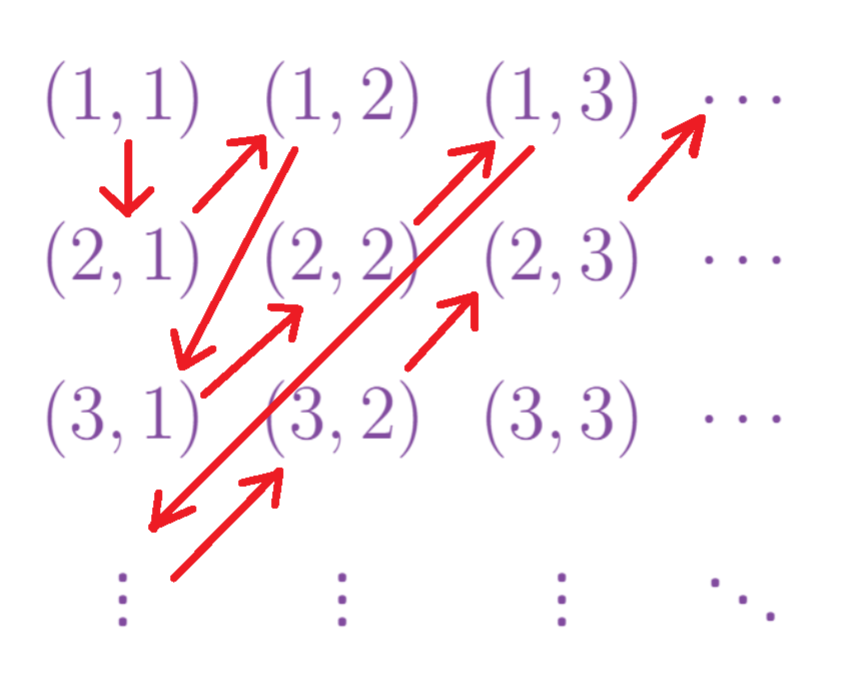
\includegraphics[scale=0.55]{Cartesian_Product_Bijection.png}
      \end{myClosureOne}
   \end{center}}
   \retTwo
   \markLecture{1/24/2024}

   {\hTwo
   \begin{myIndent}
      Proposition \propCount: If $A$ is a countable set, $B$ any set, and $g: A\rightarrow B$ is a surjection, then $B$ is countable.
      
      {\begin{myIndent} \hThree
         Proof:\\
         If $A$ is finite, then $B = g(A)$ is finite as well. So the proposition is trivially true. Now assume $A$ is infinite. Then since $A$ is countable, there is a bijection\\ $f: \mathbb{Z}^+ \rightarrow A$. Now define $\phi = g \circ f: \mathbb{Z}^+ \rightarrow B$. We know that $\phi$ is a surjection as it is the composition of two surjections. \retTwo

         Let $E \subseteq \mathbb{Z}^+$ be any set that contains precisely one element of $\phi^{-1}(b)$ for each $b\in B$. For instance, we can define $E$ as the set: \[\{n \in \mathbb{Z}^+ \mid \forall m \in \mathbb{Z}^+, \hspace{0.25em} m<n \Rightarrow \phi(m) \neq \phi(n)\}\]

         \newpage

         Now by proposition 8, we know that $E$ is countable as $E$ is a subset of a \\countable set. But additionally we have that $\phi$ acts as a bijection from $E$ to $B$. Therefore, $\lvert E \rvert = \lvert B \rvert$, meaning $B$ is countable. \retTwo
      \end{myIndent}}

      Proposition \propCount: A set $A$ is countable if and only if there exists a surjection from\\ $\mathbb{Z}^+$ onto $A$.
      {\hThree
      \begin{myIndent}
         Proof:\\
         ($\Longleftarrow$) Since $\mathbb{Z}^+$ is the definition of a countable set, if there is a surjection from $\mathbb{Z}^+$ to $A$, then we have by proposition 10 that $A$ is also countable. \retTwo

         ($\Longrightarrow$) Assume $A$ is countable. If $A$ is finite, then we can number the elements of $A$ as $\{a_1, a_2, \ldots, a_n\}$. So, we may define the surjection $f: \mathbb{Z}^+ \rightarrow A$ with the correspondance rule:
         \[f(k) = \left\{
         \begin{matrix}
            a_k \quad \text{ if } k \leq n \\
            a_n \quad \text{ if } k > n
         \end{matrix}\right.\]
         Meanwhile if $A$ is infinite, then by definition there exists a bijection from $\mathbb{Z}^+$ to $A$. So, no matter if $A$ is infinite or finite, if $A$ is countable, then there exists a bijection from $\mathbb{Z}^+$ to $A$. \retTwo
      \end{myIndent}}

      Proposition \propCount: If $E_n$ is a countable set for each $n\in\mathbb{Z}^+$, then ${\displaystyle \mathlarger{\bigcup}_{\phantom{+}n \in \mathbb{Z}^+}{E_n}}$ is countable.
      
      {\begin{myIndent} \hThree
         Proof:\\ For each $n \in \mathbb{Z}^+$, there is a surjection $f_n: \mathbb{Z}^+ \rightarrow E_n$.\\  Define $g: \mathbb{Z}^+ \times \mathbb{Z}^+ \rightarrow {\displaystyle \mathlarger{\bigcup}_{\phantom{+}n \in \mathbb{Z}^+}{E_n}} \hspace{0.1em}$ by $g(n, k) = f_n(k)$. \retTwo Then as $g$ is a surjection and $\mathbb{Z} \times \mathbb{Z}$ is countable by proposition 9, we know by proposition 10 that ${\displaystyle \mathlarger{\bigcup}_{\phantom{+}n \in \mathbb{Z}^+}{E_n}}$ is countable.
         {\begin{myTindent}\begin{myDindent} \teachComment
            In other words, the union of countably many \\countable sets is countable. \retTwo
         \end{myDindent}\end{myTindent}}
      \end{myIndent}}
      
      Proposition \propCount: If $A$ is countable, then for every $n \in \mathbb{Z}^+$, the set $A^n = A \times A \times \ldots \times A$ is countable.

      {\hThree
      \begin{myIndent}
         Proof: (we can proceed by induction) \\
         When $n=1$, then $A^n = A^1 = A$ is obviously countable.\\
         Now assume the proposition is true for $n-1$, meaning $A^{n-1}$ is countable. Then: $A^n = {\displaystyle \mathlarger{\bigcup}_{a \in A}{\{a\} \times A^{n-1}}}$ is countable by proposition 12.
      \end{myIndent}}
      \newpage

      Corollary: $\mathbb{Q}$ is countable.
      {\begin{myIndent} \hThree
         Proof:\\
         Define $f: \mathbb{Q} \rightarrow \mathbb{Z} \times \mathbb{Z}^+$ by setting $f(p) = (n, m)$ where $n, m$ are the unique coprime integers with $m>0$, $\frac{n}{m}=p$. Also define $f(0) = (1, 0)$ Then\\ $f(\mathbb{Q}) \subset \mathbb{Z} \times \mathbb{Z}^+$ and the latter set is countable. So $f(\mathbb{Q})$ is countable. Since $f$ is injective, $f$ is a bijection between $\mathbb{Q}$ and a countable set. Thus $\mathbb{Q}$ is countable. \retTwo
      \end{myIndent}}
   \end{myIndent}}
   Given sets $A$ and $B$, we write $A^B$ to denote the set of all functions from $B$ to $A$. \retTwo
   
   {\begin{myIndent} \hTwo
      Proposition \propCount: $\{0, 1\}^{\mathbb{Z}^+}$ is uncountable.
      \hThree
      \begin{myIndent}
         Proof: Let $\{f_1, f_2, \ldots\}$ be any countable subset of $\{0, 1\}^{\mathbb{Z}^+}$. Then define\\ $g \in \{0, 1\}^{\mathbb{Z}^+}$ by the rule $g(n) = 1 - f_n(n)$. Since $g(n) \neq f_n(n)$, we have that $g \neq f_n$. Since this holds for all $n \in \mathbb{Z}^+$, we can thus conclude that $g \notin \{f_1, f_2, \ldots\}$. We thus conclude that any countable subset of $\{0, 1\}^{\mathbb{Z}^+}$ is a proper subset. So $\{0, 1\}^{\mathbb{Z}^+}$ must be uncountable.
      \end{myIndent} \retTwo
   \end{myIndent}}

   \markLecture{1/26/2024}

   test
\end{document}